\documentclass{article}

\usepackage{amsmath}
\usepackage{amsfonts}
\usepackage{amssymb}
\usepackage{amsthm}
\usepackage{mathtools}
\usepackage[breakable, skins]{tcolorbox}
\usepackage[vlined]{algorithm2e}
\usepackage{hyperref}
\usepackage{graphicx}
\usepackage{float}

% make the document title look pretty fancy
\makeatletter
\renewcommand{\maketitle}{
  \begin{center}
  {\vspace*{10mm}\LARGE\@title\par}
  {\vspace{7mm}\large\@author\par}
  {\vspace{1mm}21-241 Final Project\par}
  {\vspace{3mm}\large\@date\vspace{8mm}}
  \end{center}
}
\makeatother

% set up fancy color box theorems
\tcbuselibrary{theorems}
\newtcbtheorem[number within=section]{definition}{Definition}{
  colback=red!5,
  colframe=red!35!black,
  fonttitle=\bfseries
}{defn}
\newtcbtheorem[number within=section]{theorem}{Theorem}{
  colback=blue!5,
  colframe=blue!35!black,
  fonttitle=\bfseries
}{thm}
\newtcbtheorem[number within=section]{example}{Example}{
  colback=green!5,
  colframe=green!35!black,
  fonttitle=\bfseries
}{ex}
\newtcbtheorem[number within=section]{algo}{Algorithm}{
  colback=gray!5,
  colframe=gray!35!black,
  fonttitle=\bfseries
}{algo}
\newtheorem*{remark}{Remark}

% math commands
\let\vec\mathbf
\def\store{$\leftarrow$ }

% document meta-info
\title{Numerical Methods for Computing Eigenvectors}
\author{Eric Zheng}
\date{December 6, 2019}

\begin{document}
\maketitle

\begin{abstract}
  In this document, I present some background on numerical methods for computing
  the eigenvectors and singular vectors of matrices. A Julia implementation of
  the power and QR methods is given, and the two algorithms are compared
\end{abstract}

\tableofcontents

\section{Background: Eigenvectors and Eigenvalues}
I assume that the reader is familiar with linear algebra at the college introductory level. In this section, I review a little bit of background to motivate the algorithms that will be developed in subsequent sections. We begin by recalling definition \ref{defn:eigen}.

\begin{definition}{eigenvectors and eigenvalues}{eigen}
  Consider an arbitrary $n \times n$ matrix $A$. For some $\vec{x} \in \mathbb{R}^n$ (with $\vec{x} \neq \vec{0}$), we say that $\vec{x}$ is an \textit{eigenvector} of $A$ iff, for some $\lambda \in \mathbb{R}$, $A\vec{x} = \lambda\vec{x}$. We denote $\lambda$ as the corresponding \textit{eigenvalue} of $A$.
\end{definition}

From definition \ref{defn:eigen} follows immediately a somewhat naive way to compute the eigenvalues of a given matrix. Note that
\begin{equation*}
  A\vec{x} = \lambda\vec{x} \implies A\vec{x} - \lambda\vec{x} = \vec{0}
\end{equation*}
and $\lambda\vec{x} = \lambda I \vec{x}$, so we have
\begin{equation*}
  A\vec{x} - \lambda I \vec{x} = (A - \lambda I)\vec{x} = \vec{0}.
\end{equation*}
That is to say, $\lambda \in \mathbb{R}^n$ is an eigenvalue of $A$ if and only if $A - \lambda I$ has a non-trivial null space. A matrix has a non-trivial null space if and only if it is singular, so we require that $\det(A - \lambda I) = 0$. This result is stated in theorem \ref{thm:poly}.

\begin{theorem}{computing eigenvalues as polynomial roots}{poly}
  Some $\lambda \in \mathbb{R}^n$ is an eigenvalue of the $n \times n$ matrix $A$ if and only if $\det (A - \lambda I) = 0$. We call $\det (A - \lambda I)$ the \textit{characteristic polynomial} for $A$. The problem then becomes identifying the roots of this polynomial.
\end{theorem}

Once the eigenvalues have been computed, we can find the corresponding eigenvectors by finding the null space of $A - \lambda I$, for example by using the reduced row echelon form. The key drawback of this method is that polynomial root-finding is sensitive to small numerical errors.

\begin{example}{sensitivity of polynomial root finding}{sensitivity}
  Consider the matrix
\end{example}

However, the equivalence of eigenvalue-finding and polynomial root-finding gives some insight into how we could approach the problem with more advanced methods. It is known that polynomials of degree five and higher do not in general have a solution by radicals [cite], although we can use iterative methods to get arbitrarily good approximations of these roots. In the following sections, we will apply similar iterative methodologies to find the eigenvectors and eigenvalues of matrices.

\section{The Power Method}
\subsection{Mathematical Formulation}
\begin{definition}{dominant eigenvector}{domeigen}
  Let $\lambda_1, \ldots, \lambda_n$ be the eigenvalues of the matrix $A$, and let $\vec{x}_1, \ldots, \vec{x}_n$ be corresponding eigenvalues. We call $\vec{x}_i$ a \textit{dominant eigenvector} if $|\lambda_i| > |\lambda_j|$ whenever $i \neq j$. The corresponding $\lambda_i$ is called the \textit{dominant eigenvalue}.
\end{definition}

The power method for computing eigenvectors takes successive powers of the matrix $A^k$ until some stopping criterion is reached. As $k$ grows large, the columns of $A$ will approach the dominant eigenvector of $A$. This is stated in theorem \ref{thm:powermethod}.

\begin{theorem}{the power method}{powermethod}
  If $A$ is an $n \times n$ diagonalizable matrix with a dominant eigenvector $\vec{x}$, then the columns of $A^k$ approach a multiple of $\vec{x}$ as $k$ grows arbitrarily large. (More precisely, at least one column does so.)
\end{theorem}
\begin{proof}
  Since $A$ is diagonalizable, let $\vec{x}_1, \ldots, \vec{x}_n$ be a basis of eigenvectors for $\mathbb{R}^n$, where we order the eigenvectors so that $\vec{x}_1$ is a dominant eigenvector. Now since the $\vec{x}_i$'s form a basis, any $\vec{v} \in \mathbb{R}^n$ can be expressed as the linear combination
  \begin{equation*}
    \vec{v} = c_1\vec{x}_1 + \cdots + c_n\vec{x}_n.
  \end{equation*}
  Then by linearity, we have
  \begin{align*}
    A^k\vec{v} &= A^k(c_1\vec{x}_1 + \cdots + c_n\vec{x}_n) \\
               &= A^kc_1\vec{x}_1 + \cdots + A^kc_n\vec{x}_n \\
               &= \lambda_1^kc_1\vec{x}_1 + \cdots + \lambda_n^kc_n\vec{x}_n.
  \end{align*}
  But since $|\lambda_1| > |\lambda_i|$ for all $i \geq 2$, we see that the first term $\lambda_1^kc_1\vec{x}_1$ dominates as $k$ grows very large (as long as $c_1 \neq 0$). Hence for large $k$, $A^k\vec{v} \approx \lambda_1^kc_1\vec{x}_1$, if $c_1 \neq 0$. Taking $\vec{v}$ to be the standard basis vectors then produces the desired result, since at least one of the $\vec{e}_i$'s must have a component along $\vec{x}_1$.
\end{proof}

One issue with the power method is that it assumes that $A$ is both diagonalizable and has a dominant eigenvector. These flaws are highlighted in examples \ref{ex:powernodiag} and \ref{ex:powernodom}. Another example of the power method's failure to converge is a rotation matrix \cite{pwr-rot}, which does not typically have real eigenvalues.

\begin{example}{power method on a non-diagonalizable matrix}{powernodiag}
  The power method can fail when a matrix is not diagonalizable. Consider the matrix
  \begin{equation*}
    A = \begin{bmatrix}0 & 1 \\ 0 & 0\end{bmatrix}.
  \end{equation*}
  $A$ has eigenvalue $\lambda = 0$ with eigenvector $(1, 0)$. But $A$ is nilpotent, so the columns of $A^k$ will never approach a multiple of $(1, 0)$.

  ACTUALLY...rotation matrix might be a better example, since this can be thought of more as a failure around zero (i.e. $(0,0)$ is a legitimate multiple of $(1,0)$)
\end{example}

\begin{example}{power method without a dominant eigenvalue}{powernodom}
  The power method can fail when a matrix does not have a dominant eigenvalue, even if it is diagonalizable. Consider the matrix
  \begin{equation*}
    A = \begin{bmatrix}0 & 1 \\ 1 & 0\end{bmatrix}.
  \end{equation*}
  Now $A$ is clearly diagonalizable (it's already diagonal), but its eigenvalues are $\lambda = \pm 1$, so $A$ does not have a dominant eigenvalue. If we attempt the power method, we find that $A^2 = I$, so the successive powers $A^k$ will oscillate between $A$ (when $k$ is odd) and $I$ (when $k$ is even). Neither of these contain the eigenvectors of $A$, which are $(1,1)$ and $(1,-1)$.
\end{example}

Note that diagonalizability is a sufficient condition for the power method to converge (when combined with a dominant eigenvalue), but it is not necessary. Example \ref{ex:powerworksnodiag} gives a matrix that is not diagonalizable yet converges under the power method.

\begin{example}{power method despite non-diagonalizability}{powerworksnodiag}
  Consider the matrix
  \begin{equation*}
    A = \begin{bmatrix}1 & 0 \\ 1 & 1\end{bmatrix}.
  \end{equation*}
  This matrix has only one eigenvalue $\lambda = 1$ with eigenvectors $(0,1)$ and $(0,-1)$, which are not independent. But an easy induction reveals that
  \begin{equation*}
    A^k = \begin{bmatrix}1 & 0 \\ k & 1\end{bmatrix}
  \end{equation*}
  whose columns indeed converge to the eigenvector $(0, 1)$ as $k$ grows large.
\end{example}

\subsection{Convergence Analysis}
The power method is a particularly elegant method for computing the dominant eigenvector of a matrix, but how efficient is it? In other words, as we take successive powers $A^k$, how quickly does $\lambda_1$ dominate the result? What matters here is comparatively how much larger $|\lambda_1|$ is than $|\lambda_2|$: the power method converges proportional to $|\lambda_1 / \lambda_2|$ \cite[p.~529]{strang}.

More formally, we can prove this by an argument taken from \cite{mit-sensitivity}: if $A$ is diagonalizable, then we can express any $\vec{v} \in \mathbb{R}^n$ as
\begin{equation*}
  \vec{v} = c_1\vec{x}_1 + c_2\vec{x}_2 + \cdots + c_n\vec{x}_n
\end{equation*}
where we assume $c_1 \neq 0$ for the algorithm to converge. Now after $k$ steps, we have
\begin{align*}
  A^k\vec{v} &= \lambda_1^k c_1\vec{x}_1 + \lambda_2^k c_2\vec{x}_2 + \cdots + \lambda_n^k c_n\vec{x}_n \\
             &= \lambda_1^k \left[c_1\vec{x}_1 + \left(\frac{\lambda_2}{\lambda_1}\right)^k c_2\vec{x}_2 + \cdots + \left(\frac{\lambda_n}{\lambda_1}\right)^k c_n\vec{x}_n\right]
\end{align*}
where $|\lambda_i / \lambda_1| < 1$ whenever $i \ge 2$ since $\lambda_1$ is the dominant eigenvalue. Now as $k \to \infty$, the $(\lambda_2 / \lambda_1)$ term will dominate the error, so we expect the algorithm to converge proportionally to $|\lambda_2 / \lambda_1|^k$.

We can test this numerically with the matrix
\begin{equation*}
  A = \begin{bmatrix}23 & 5 & 2 \\ 5 & 23 & 2 \\ 2 & 2 & 26\end{bmatrix}
\end{equation*}
which has eigenvalues $\lambda_1 = 30$, $\lambda_2 = 24$, and $\lambda_3 = 18$; the corresponding eigenvectors are $\vec{x}_1 = (1,1,1)$, $\vec{x}_2 = (1,1,-2)$, and $\vec{x}_3 = (1,-1,0)$. For the first twenty iterations of the power method, we get something like figure \ref{powermethod-plot}, which is fairly close to the expected $(24/30)^k = (4/5)^k$ decay rate. The Julia code for generating the plot is included in the appendix.

\begin{figure}[H]
  \begin{center}
    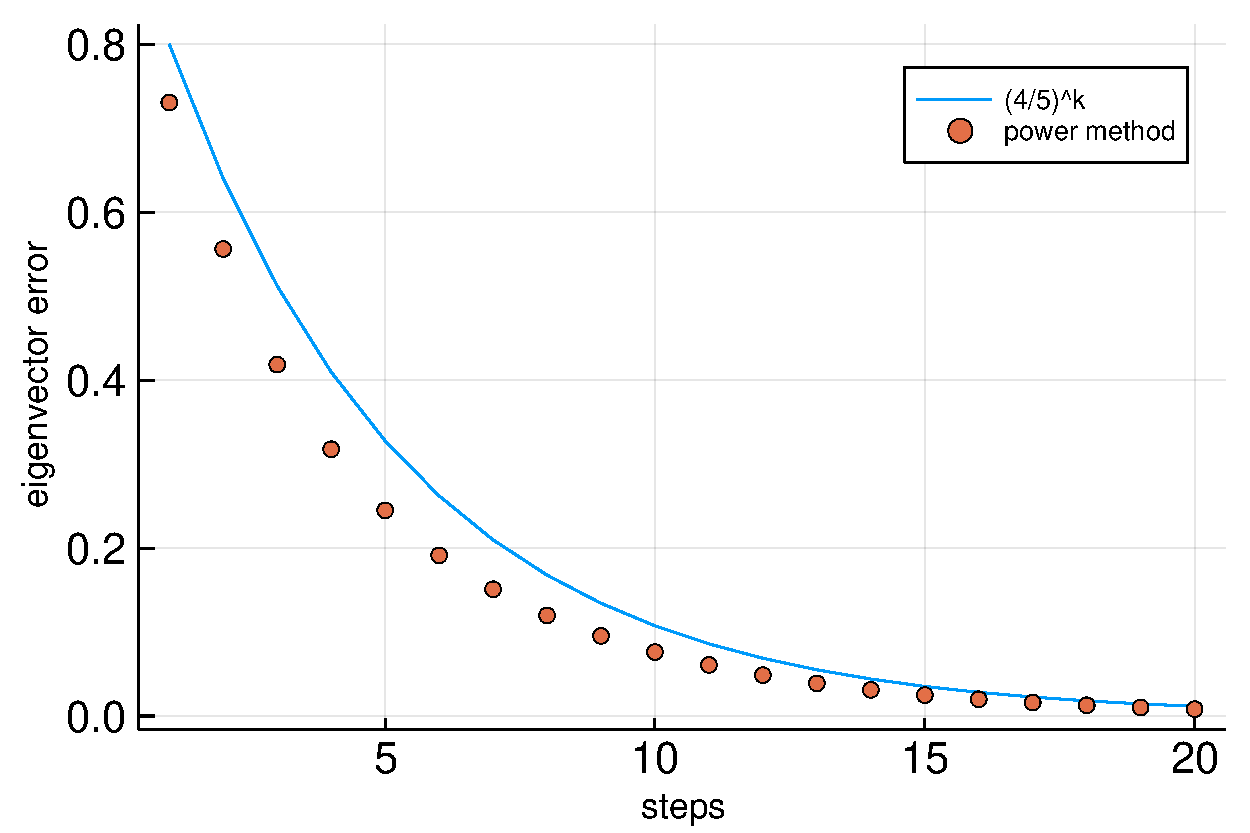
\includegraphics[width=0.75\textwidth]{power-method.pdf}
    \caption{Power method error for twenty steps of the algorithm, plotted against the expected error given by $|\lambda_2 / \lambda_1|^k$}
    \label{powermethod-plot}
  \end{center}
\end{figure}

\subsection{Rayleigh Quotients}
Up until now, we have developed a method for finding the eigenvectors of a matrix, but what about the eigenvalues? Based on definition \ref{defn:eigen}, it is tempting to just take an eigenvector $\vec{x} \in \mathbb{R}^n$, compute $A\vec{x} = \lambda\vec{x}$, and then see how much the components of $\vec{x}$ were scaled to find $\lambda$.

The issue is that our algorithm only generates an approximation to $\vec{x}$, not $\vec{x}$ itself \footnote{In fact, even if we gave the algorithm infinite time to run, it is mathematically impossible for a computer with a finite alphabet to represent arbitrary reals, since $\mathbb{R}$ is uncountable.}. Hence each of the components will not be exactly scaled by $\lambda$: some might be a little larger than they should be, and some might be a little smaller. The next thing that comes to mind is to let $\mu_i$ be the amount by which each component of $\vec{x}$ was scaled and then just average the $\mu_i$'s. Unfortunately, this approach is sensitive to small errors, particularly around $0$ \cite{mit-sensitivity}, as demonstrated in example \ref{ex:naive-eigen-avg}.

\begin{example}{sensitivity of averaging for finding $\lambda$}{naive-eigen-avg}
  Consider the matrix
  \begin{equation*}
    A = \begin{bmatrix}2 & 0 \\ 0 & 1\end{bmatrix}
  \end{equation*}
  which has $\vec{x}_1 = (1,0)$ and $\vec{x}_2 = (0,1)$ with corresponding $\lambda_1 = 2$ and $\lambda_2 = 1$. Now suppose we have an eigenvector approximation $\hat{\vec{x}}_1 = (1, 0.00001)$. This is very close to the true dominant eigenvector:
  \begin{equation*}
    \lVert \hat{\vec{x}}_1 - \vec{x}_1 \rVert = 0.00001,
  \end{equation*}
  yet we have
  \begin{equation*}
    A\hat{\vec{x}}_1 = \begin{bmatrix}2 & 0 \\ 0 & 1\end{bmatrix}\begin{bmatrix}1 \\ 0.00001\end{bmatrix} = \begin{bmatrix}2 \\ 0.00001\end{bmatrix}.
  \end{equation*}
  If we try to approximate $\lambda_1$ by diving component-wise and then averaging, we get:
  \begin{align*}
    \mu_1 &= 2 / 1 = 2 \\
    \mu_2 &= 0.00001 / 0.00001 = 1
  \end{align*}
  which would give $\lambda \approx 3/2$, which is significantly off from the true value $\lambda = 2$, despite the very good eigenvector approximation.
\end{example}

So how should we compute eigenvalues given a corresponding eigenvector? A common way to do this is via the Rayleigh quotient, given in definition \ref{defn:rayleigh}.

\begin{definition}{Rayleigh quotient CITE}{rayleigh}
  If we have an approximation $\vec{x} \in \mathbb{R}^n$ for an eigenvector of $A$, then the \textit{Rayleigh quotient} approximation for the corresponding eigenvalue $\lambda$ is given by
  \begin{equation*}
    \lambda \approx \frac{\vec{x}^TA\vec{x}}{\vec{x}^T\vec{x}}.
  \end{equation*}
\end{definition}

This can be thought of as the average of the $\mu_i$'s weighted by the square of each component \cite{mit-sensitivity}, so errors around small components affect the overall eigenvalue approximation very little. For example, using the same numbers as example \ref{ex:naive-eigen-avg}, we get
\begin{equation*}
  \lambda \approx \frac{\hat{\vec{x}}_1^T A \hat{\vec{x}}_1}{\hat{\vec{x}}^T\hat{\vec{x}}} = \frac{2.0000000001}{1.0000000001} \approx 1.999999999
\end{equation*}
which is much closer to the true value of $\lambda = 2$.

\subsection{Deflation}
One limitation is that the power method, as presented in theorem \ref{thm:powermethod}, only finds the dominant eigenvector of a matrix. For many physical systems, the behavior is determined mostly by the dominant eigenvector, so this is sufficient \cite{spanish}. However, in the special case where $A$ is symmetric, we can actually do better. By the spectral theorem (restated in theorem \ref{thm:spectral}), we can take the spectral decomposition of symmetric $A$ into orthogonal $X$ and diagonal $\Lambda$, as in
\begin{equation*}
  A = X \Lambda X^T = \lambda_1 \vec{x}_1 \vec{x}_1^T + \cdots + \lambda_n \vec{x}_n \vec{x}_n^T
\end{equation*}
where we sort the eigenvalues in order of magnitude. Now applying the power method will yield $\vec{x}_1$ (which in turn can be used to find $\lambda_1$). But observe that
\begin{equation*}
  B_1 = A - \lambda_1 \vec{x}_1 \vec{x}_1^T = \lambda_2 \vec{x}_2 \vec{x}_2^T + \cdots + \lambda_n \vec{x}_n \vec{x}_n^T
\end{equation*}
is a symmetric matrix that has eigenvalues $\lambda_2, \ldots, \lambda_n$ and corresponding $\vec{x}_2, \ldots, \vec{x}_n$! ($B_1$ also has a zero eigenvalue, which is not important because it is the least in magnitude.) Hence we can apply the power method to $B_1$ to find $\vec{x}_2$ and $\lambda_2$. We can keep on going with
\begin{equation*}
  B_2 = B_1 - \lambda_2 \vec{x}_2 \vec{x}_2^T = \lambda_3 \vec{x}_3 \vec{x}_3^T + \cdots + \lambda_n \vec{x}_n \vec{x}_n^T
\end{equation*}
to which we can apply the power method to pick off $\vec{x}_3$ and $\lambda_3$. We keep on going until we have found all $n$ eigenvectors, a technique known as \textit{deflation}.

In fact, even if $A$ is not symmetric, we can apply a similar deflation technique for finding all the eigenvalues of $A$, although we don't get any additional eigenvectors beyond the dominant one. The reader is referred to \cite{deflation} for a full explanation, but a more general deflation procedure known as Hotelling's deflation is given in theorem \ref{thm:hotelling-deflation}. In the case when we take unit eigenvectors of a symmetric matrix, this procedure becomes the previously described deflation procedure. There exist other techniques that are even more robust against, for instance, rounding errors \cite{deflation-robots}, but they are beyond the scope of this paper.

\begin{theorem}{Hotelling's deflation}{hotelling-deflation}
  Suppose $A$ is a matrix with eigenvalues $\lambda_1, \ldots, \lambda_k$ and corresponding eigenvalues $\vec{x}_1, \ldots, \vec{x}_k$. Then the matrix
  \begin{equation*}
    B = A - \frac{\lambda_1}{\vec{x}_1^T\vec{x}}\vec{x}_1\vec{x}_1^T
  \end{equation*}
  has eigenvalues $\lambda_2, \ldots, \lambda_k$, although it does not necessarily have the same eigenvectors $\vec{x}_2, \ldots, \vec{x}_k$.
\end{theorem}

\subsection{Optimization for Sparse Matrices}
As we have developed it thus far, the power method involves computing large powers $A^k$. While we can make this somewhat efficient via tricks like exponentiation by squaring, matrix multiplication is an expensive thing to do; the best known algorithms run in roughly $O(n^{2.373})$ \cite{matmul} for an $n \times n$ matrix. Can we do better?

A faster approach is to reframe the problem as a bunch of matrix-vector multiplications, which can be computed naively in $O(n^2)$. In fact, if $A$ is a sparse matrix (i.e. most entires are zero), matrix-vector multiplication can become \emph{extremely} efficient \cite{pwr-rot}. We can tweak theorem \ref{thm:powermethod} slightly into theorem \ref{thm:powermethod-sparse}, whose proof is much the same as theorem \ref{thm:powermethod}.

\begin{theorem}{more efficient power method}{powermethod-sparse}
  Suppose $A$ is an $n \times n$ diagonalizable matrix with a dominant eigenvalue $\lambda$ and corresponding eigenvector $\vec{x}$. Then there exists some $\vec{v}_0 \in \mathbb{R}^n$ such that
  \begin{equation*}
    \vec{v}_k = A^k\vec{v}_0 = A\vec{v}_{k-1}
  \end{equation*}
  approaches a multiple of $\vec{x}$ as $k$ grows arbitrarily large.
\end{theorem}

Now if $A$ is diagonalizable, then any $\vec{v}_0 \in \mathbb{R}^n$ can be expressed in the basis of eigenvectors as
\begin{equation*}
  \vec{v}_0 = c_1\vec{x}_1 + \cdots + c_n\vec{x}_n.
\end{equation*}
As long as $\vec{v}_0$ has some component $c_1 \neq 0$ along $\vec{x}_1$, then $A^k\vec{v}_0$ will converge to $\vec{x}_1$ as $k$ grows large. This is great, since $A^k\vec{v}_0$ can be recursively computed as $A(A^{k-1}\vec{v}_0)$, which is $k$ matrix-vector multiplications instead of $k$ matrix-matrix multiplications.

But what happens if we choose an initial vector $\vec{v}_0$ with $c_1 = 0$? In this case, it is possible that this method will fail to converge. An example is given in example \ref{ex:power-sparse-no-convergence}. However, if we just choose a random $\vec{v}_0 \in \mathbb{R}^n$, we get $c_1 \neq 0$ with very high probability \cite[p.~53]{cornell}, so this is not particularly worrisome. Additionally, even if we are incredibly unlucky and choose a $\vec{v}_0$ that is deficient in $\vec{x}_1$, rounding errors in the computations will likely save us and push so that $c_1 \neq 0$ \cite{pwr-rot}.

\begin{example}{efficient power method with bad $\vec{v}_0$}{power-sparse-no-convergence}
  Consider the matrix
  \begin{equation*}
    A = \begin{bmatrix}11 & 5 & 2 \\ 5 & 11 & 2 \\ 2 & 2 & 14\end{bmatrix}
  \end{equation*}
  which has eigenvalues $\lambda_1 = 18$, $\lambda_2 = 12$, $\lambda_3 = 6$ with corresponding eigenvectors $\vec{x}_1 = (1,1,1)$, $\vec{x}_2 = (1,1,-2)$, and $\vec{x}_3 = (1,-1,0)$. If we choose a good initial vector like $\vec{v}_0 = (1,2,3)$, we indeed get
  \begin{equation*}
    \vec{v}_k \to a\vec{x}_1 \textrm{  as  } k \to \infty.
  \end{equation*}
  However, if we instead choose a bad initial vector like $\vec{v}_0 = (1,0,-1)$ (which is orthogonal to $\vec{x}_1$), we instead get $\vec{v}_k \to b\vec{x}_2$. In this case, since $A$ was diagonalizable, we still ended up with an eigenvector of $A$ (just not the one we expected). If we instead had a non-diagonalizable matrix like
  \begin{equation*}
    B = \begin{bmatrix}2 & 0 & 0 \\ 0 & 0 & -1 \\ 0 & 1 & 0\end{bmatrix},
  \end{equation*}
  which has real eigenvalue $\lambda=2$ and $\vec{x} = (1,0,0)$, we could fail to converge to anything at all if we choose $\vec{v}_0 = (0,1,1)$. However, a good choice of $\vec{v}_0 = (1,1,1)$ will still converge to a multiple of $\vec{x}$, highlighting the importance of the initial vector selection.
\end{example}

\subsection{Implementation}
Based on the power method (as presented in theorem \ref{thm:powermethod}), we present algorithm \ref{algo:domeigen} to compute the dominant eigenvector and eigenvalue of a given diagonalizable matrix. The algorithm may also converge for a non-diagonalizable matrix, but we do not guarantee this. The referenced subroutine \texttt{FirstNonzeroCol} gets the first nonzero column of the given matrix (or the first whose norm exceeds some tolerance), and $\texttt{SquareAndNorm}$ takes a given matrix $A$ and then returns $A^2$, normalized by the magnitude of its first nonzero column.

In this implementation of the power method, we choose to compute $A^{2k} = A^kA^k$ rather than $A^{k+1} = A^kA$ at step $k$ because this is just as efficient (i.e. an $n \times n$ matrix multiplication) yet produces larger powers and therefore converges faster.

\begin{algo}{\texttt{DominantEigen1}}{domeigen}
  \begin{algorithm}[H]
    \SetKwInOut{Input}{input}
    \SetKwInOut{Parameter}{parameter}
    \SetKwInOut{Output}{output}
    \SetKwFunction{FirstNonzeroCol}{FirstNonzeroCol}
    \SetKwFunction{SquareAndNorm}{SquareAndNormalize}

    \Input{real diagonalizable $n \times n$ matrix $A$}
    \Parameter{tolerance $\varepsilon > 0$, max iterations $N > 0$}
    \Output{dominant eigenpair $(\vec{x}, \lambda)$}
    \BlankLine
    $A'$ \store $A$\;
    $i$ \store $0$\tcp*{number of iterations so far}
    $\vec{x}$ \store \FirstNonzeroCol{$A'$}\;
    $A'$ \store \SquareAndNorm{$A'$}\;
    \While{$\lVert\vec{x} - \FirstNonzeroCol{$A'$}\rVert > \varepsilon$ {\normalfont and} $i < N$}{
      $\vec{x}$ \store \FirstNonzeroCol{$A'$}\;
      $A'$ \store \SquareAndNorm{$A'$}\;
      $i$ \store $i + 1$\;
    }
    $\vec{x}$ \store \FirstNonzeroCol{$A'$}\;
    $\lambda$ \store $(\vec{x}^TA\vec{x}) / (\vec{x}^T\vec{x})$\;
  \end{algorithm}
\end{algo}

Additionally, based on theorem \ref{thm:powermethod-sparse}, we implement the more efficient power method as algorithm \ref{algo:domeigen2}.

\begin{algo}{\texttt{DominantEigen2}}{domeigen2}
  \begin{algorithm}[H]
    \SetKwInOut{Input}{input}
    \SetKwInOut{Parameter}{parameter}
    \SetKwInOut{Output}{output}
    \SetKwFunction{Normalize}{Normalize}

    \Input{real diagonalizable $n \times n$ matrix $A$}
    \Parameter{tolerance $\varepsilon > 0$, max iterations $N > 0$}
    \Output{dominant eigenpair $(\vec{x}, \lambda)$}
    \BlankLine
    $\vec{x}$ \store choose random vector in $\mathbb{R}^n$\;
    $\vec{x}$ \store \Normalize{$\vec{x}$}\;
    $i$ \store $0$\tcp*{number of iterations so far}
    \While{$\lVert A\vec{x} - \vec{x}\rVert > \varepsilon$ {\normalfont and } $i < N$}{
      $\vec{x}$ \store \Normalize{$A\vec{x}$}\;
      $i$ \store $i + 1$\;
    }
    $\lambda$ \store $(\vec{x}^TA\vec{x}) / (\vec{x}^T\vec{x})$\;
  \end{algorithm}
\end{algo}

Finally, we can use the deflation method from theorem \ref{thm:hotelling-deflation} to write a general power method routine (algorithm \ref{algo:pwrsym}) that computes all the eigenvectors and eigenvalues of a symmetric matrix.

\begin{algo}{\texttt{EigenPowerSymmetric}}{pwrsym}
  \begin{algorithm}[H]
    \SetKwInOut{Input}{input}
    \SetKwInOut{Parameter}{parameter}
    \SetKwInOut{Output}{output}
    \SetKwFunction{DominantEigen}{DominantEigen}

    \Input{real symmetric $n \times n$ matrix $S$}
    \Parameter{tolerance $\varepsilon > 0$, max iterations $N > 0$}
    \Output{list $xs$ of eigenvectors and $\lambda s$ of eigenvalues}
    \BlankLine
    $xs$ $\leftarrow$ empty list\;
    $\lambda s$ $\leftarrow$ empty list\;
    \For{$i \in [n]$}{
      $\vec{x}$, $\lambda$ $\leftarrow$ \DominantEigen{$S$}\;
      $S$ \store $S - (\lambda/(\vec{x}^T\vec{x}))\vec{x}\vec{x}^T$\;
      append $\vec{x}$ to $xs$\;
      append $\lambda$ to $\lambda s$\;
    }
  \end{algorithm}
\end{algo}

\section{The QR Method}
\subsection{Mathematical Formulation}
Another iterative method to compute the eigenvalues of a matrix is known as the $QR$ method. The key insight behind this method is that similar matrices have the same eigenvalues, a fact proven in theorem \ref{thm:similar}.

\begin{theorem}{similar matrices have the same eigenvalues}{similar}
  Suppose $A$ and $C$ are similar square matrices. Then if $\lambda \in \mathbb{R}$ is an eigenvalue of $A$ if and only if it is an eigenvalue of $C$.
  
\end{theorem}
\begin{proof}
  Suppose $A = BCB^{-1}$. Now consider an eigenvalue $\lambda$ of $A$ with eigenvector $\vec{x}$. Then
  \begin{equation*}
    A\vec{x} = \lambda\vec{x} \implies BCB^{-1}\vec{x} = \lambda\vec{x}.
  \end{equation*}
  But $B$ is invertible, so we can multiply on the left by $B^{-1}$ to obtain:
  \begin{equation*}
    B^{-1}BCB^{-1} = B^{-1}(\lambda\vec{x}) \implies C(B^{-1}\vec{x}) = \lambda(B^{-1}\vec{x}).
  \end{equation*}
  Now since $B^{-1}$ is invertible, $B^{-1}\vec{x} \neq \vec{0}$ if $\vec{x} \neq 0$ (i.e. $B^{-1}$ has a trivial null space), which means that we have found an eigenvector $B^{-1}\vec{x}$ of $C$ with eigenvalue $\lambda$. An identical argument in the other direction shows that any eigenvalue of $C$ is also an eigenvalue of $A$, which concludes the proof.
\end{proof}

Additionally, recall that the eigenvalues of a triangular matrix lie on its diagonal \cite[p.~294]{strang}. (This follows from the fact that $\det(A - \lambda I) = 0$ and the determinant of triangular $A$ is the product of the diagonal entries.) This fact, combined with theorem \ref{thm:similar}, suggests the following method \cite[p.~530]{strang} of computing the eigenvalues of $A$:
\begin{enumerate}
  \item Somehow transform $A$ into a similar triangular matrix $B$.
  \item Read the eigenvalues off of the diagonal entires of $B$.
\end{enumerate}
This is not exactly the QR method, but it captures much of the intuition behind the QR method, which is presented in theorem \ref{thm:qr}.

\begin{theorem}{the QR method \cite[p.~530]{strang}}{qr}
  Suppose we have the matrix $A$. We form the sequence
  \begin{align*}
    A_0 &= A, \quad A_0 = Q_0R_0 \\
    A_1 &= R_0Q_0, \quad A_1 = Q_1R_1 \\
    A_2 &= R_1Q_1, \quad A_2 = Q_2R_2 \\
    \vdots
  \end{align*}
  which essentially takes the QR decomposition of $A_k$ at each step and reverses the factors to find the next $A_{k+1}$. In many cases, as $k \to \infty$, the $A_k$'s approach an upper triangular matrix that is similar to $A$.
\end{theorem}
\begin{proof}
  It is not always true that the $A_k$'s tend to a triangular matrix, but it is always true that $A_k$ is similar to $A$. To show this, let $A = QR$ and $A_1 = RQ$ for orthogonal $Q$ and triangular $R$. But note that
  \begin{equation*}
    QA_1Q^T = QRQQ^T = QR = A
  \end{equation*}
  so there exists a matrix $B$ such that $A = BA_1B^{-1}$, namely $B = Q^T$. At each step, the new $A_{k+1}$ is similar to the previous $A_k$, as desired.
\end{proof}

The basic QR method, as presented in theorem \ref{thm:qr}, does not always converge. An example of this, taken from \cite{cornell-qr}, is given in example \ref{ex:qr-fail}.

\begin{example}{QR algorithm failure}{qr-fail}
  Consider the matrix
  \begin{equation*}
    A = \begin{bmatrix}0 & 1 \\ 1 & 0\end{bmatrix}
  \end{equation*}
  which permits the QR decomposition
  \begin{equation*}
    Q = \begin{bmatrix}0 & 1 \\ 1 & 0\end{bmatrix}, \quad\quad
    R = \begin{bmatrix}1 & 0 \\ 0 & 1\end{bmatrix}.
  \end{equation*}
  But $A' = RQ = A$, so the algorithm gets stuck and does not converge to a triangular matrix at all.
\end{example}

There are more advanced techniques for shifting the $A_k$'s to improve the algorithm's convergence, but they are somewhat beyond the scope of this paper. The basic QR method is the basis for many

[address the thing with QR ordinarily requiring independent columns, perhaps use example [1 0 ; 1 0]]

\subsection{Going from Eigenvalues to Eigenvectors}
The QR method, as presented in theorem \ref{thm:qr}, will find all of the eigenvalues of $A$, but now we are faced with the opposite problem that we had with the power method: how do we go from eigenvalues to the corresponding eigenvectors? Of course, by definition $\vec{x} \in N(A - \lambda I)$, so we could use elimination to get the reduced row echelon form of $A - \lambda I$ and thus the null space, but is there a more sophisticated technique we could employ?

One way we could do it is the inverse power method. This method relies on a few key observations [POSSIBLY PROVE...not too hard, but time?]:
\begin{itemize}
  \item $A$ and $A - \mu I$ have the same eigenvectors.
  \item If the $\lambda_i$'s are the eigenvalues of $A$, then $1/(\lambda_i - \mu_i$'s are the eigenvalues of $A - \mu I$.
  \item $(A - \mu I)$ and $(A - \mu I)^{-1}$ have the same eigenvectors but reciprocal eigenvalues. (In general, as long as $\mu$ is not an eigenvalue of $A$, $A - \mu I$ will be invertible, since $\det(A - \mu I) \neq 0$ if $\mu$ is not an eigenvalue.)
\end{itemize}
Suppose we have the eigenvalues $\lambda_1, \ldots, \lambda_n$ of $A$, and we wish to find the eigenvector corresponding to, say, $\lambda_1$. We can take some $\mu$ that is closer to $\lambda_1$ than it is to all the other eigenvalues but is not an eigenvalue itself. Then $(A - \mu I)$

The advantage of the QR method is that it does not suffer from the rounding errors that deflation-based methods do. However, it is also not as efficient, especially in many practical scenarios where we have large systems and only care about the most dominant eigenvectors. [cite last slide in that PPT, unless I get a better source]

\subsection{Implementation}
The QR method from theorem \ref{thm:qr} can be more or less directly transcribed into an algorithm:

\begin{algo}{\texttt{EigenQR}}{qr}
  \begin{algorithm}[H]
    \SetKwInOut{Input}{input}
    \SetKwInOut{Parameter}{parameter}
    \SetKwInOut{Output}{output}
    \SetKwFunction{QRDecomposition}{QRDecomposition}

    \Input{real $n \times n$ matrix $A$}
    \Parameter{tolerance $\varepsilon > 0$, max iterations $N > 0$}
    \Output{eigenvalues $\lambda s$}
    \BlankLine
    $Q,R$ \store \QRDecomposition{$A$}\;
    $A'$ \store $RQ$\;
    $i$ \store $0$\tcp*{number of iterations so far}
    \While{$\lVert A' - A\rVert > \varepsilon$ {\normalfont and } $i < N$}{
      $Q,R$ \store \QRDecomposition{$A'$}\;
      $A$ \store $A'$\;
      $A'$ \store $RQ$\;
      $i$ \store $i + 1$\;
    }
    $\lambda s$ \store diagonal entries of $A'$\;
  \end{algorithm}
\end{algo}

\section{Connection to Singular Vectors}
Up until now, we have been almost exclusively concerned with finding the eigenvectors and eigenvalues of a matrix. But what about finding the singular vectors of a matrix?

Note that the singular vectors of any $m \times n$ matrix $A$ are just the eigenvectors of $A^TA$, so by finding the eigenvectors we already have a procedure for finding the singular vectors. To make the connection even better, note that $A^TA$ is symmetric, so by theorem \ref{thm:spectral} it is in fact diagonalizable. We can thus reliably use the power method to find both the eigenvectors and eigenvalues of $A^TA$, which give us the singular vectors and values of $A$.

\begin{theorem}{spectral theorem for real symmetric matrices}{spectral}
  If $A$ is a real symmetric $n \times n$ matrix, then $A$ has $n$ orthonormal eigenvectors. The reader is referred to [cite] for a full proof of this theorem.
\end{theorem}

\section{Algorithm Comparison}
Maybe make a table comparing power and QR, and add in some pretty graphs

\section{Appendix: Julia Code Samples}
In this appendix, I provide Julia implementations for the major algorithms presented. The Julia code for generating the plots in this paper is also included.

We first present algorithm \ref{algo:pwrsym} for symmetric matrices only because it is highly illustrative. Additionally, [all we need for singular vectors]

We square and then normalize by the first nonzero column of $A^n$. If such a column does not exist (i.e. $A^n$ is the zero matrix), then $A$ must have been a nilpotent matrix. In this case, the only eigenvalue can be zero, as proved in theorem \ref{thm:nilpotent}. In this case, the problem reduces to finding the null space of $A$.

Now a matrix can have at most $n$ independent eigenvectors, so we only have to iterate up to $n$.

\begin{theorem}{eigenvalues of a nilpotent matrix}{nilpotent}
  If $A$ is a nilpotent matrix (i.e. $A^n$ is the zero matrix for some $n \in \mathbb{N}^+$), then the only eigenvalue of $A$ is $\lambda = 0$.
  \begin{proof}
    Suppose $\vec{x} \neq \vec{0}$ were an eigenvector of $A$ with eigenvalue $\lambda \neq 0$. Then $A^n\vec{x} = \lambda^n\vec{x}$, but if $\lambda \neq 0$, then this is some nonzero vector. However, $A^n = 0$, so we also have $A^n\vec{x} = \vec{0}$, a contradiction.
  \end{proof}
\end{theorem}

Algorithm \ref{algo:pwrsym} also gives us an easy way to compute the singular values and singular vectors of any real matrix $A$: simply apply $\textrm{\texttt{EigenPowerSymmetric}}(A^TA)$.

Finding the eigenvectors of a general square matrix (not necessarily symmetric) is somewhat trickier. We will

[probably put a disclaimer at the top that we will only concern ourselves with real matrices, although we will sometimes emphasize this point in our algorithms. should we permit complex eigenvalues? nah, that moves us from Rn to Cn]

\begin{example}{failure of the power method}{pwrfail}
  The power method can fail when the original matrix does not have a dominant eigenvalue. For example, consider the matrix
  \begin{equation*}
    A = \begin{bmatrix}0 & 1 \\ 1 & 0\end{bmatrix}
  \end{equation*}
  which has eigenvalues $\lambda = \pm 1$.
\end{example}

\begin{example}{another failure of the power method}{pwrfail2}
  The power method can also fail when the original matrix has complex eigenvalues. For example, consider the matrix
  \begin{equation*}
    A = \begin{bmatrix}0 & -1 & 0 \\ 1 & 0 & 0 \\ 0 & 0 & 1\end{bmatrix}
  \end{equation*}
  which is intuitively a rotation around the $z$-axis. In this case, there is only one real eigenvalue, $\lambda=1$. If we choose a good initial $\vec{x}_0 = (0,0,1)$, the algorithm does converge to the correct solution.
\end{example}

\subsection{The QR Algorithm}

\begin{algo}{\texttt{Singular}}{singular}
  \begin{algorithm}[H]
    \SetKwInOut{Input}{input}
    \SetKwInOut{Parameter}{parameter}
    \SetKwInOut{Output}{output}
    \SetKwFunction{EigenPowerSymmetric}{EigenPowerSymmetric}

    \Input{real $m \times n$ matrix $A$}
    \Parameter{tolerance $\varepsilon > 0$, max iterations $N > 0$}
    \Output{list of singular vectors $vs$ and singular values $\sigma s$}
    \BlankLine
    \tcc{here we use the power method, but we could also use the QR method}
    $xs$, $\lambda s$ \store \EigenPowerSymmetric{$A^TA$}\;
    $\sigma s$ \store filter positive $\lambda s$\;
    $l$ \store length of $\sigma s$\;
    $vs$ \store first $l$ of $xs$\;
    \Return{$vs$, $\sigma s$}
  \end{algorithm}
\end{algo}


\begin{thebibliography}{9}
  \bibitem{pwr-rot} \url{https://www.cs.huji.ac.il/\~csip/tirgul2.pdf}
  \bibitem{mit-sensitivity} \url{https://web.mit.edu/18.06/www/Spring17/Power-Method.pdf}
  \bibitem{deflation} \url{http://www.macs.citadel.edu/chenm/344.dir/08.dir/lect4_2.pdf}
  \bibitem{matmul} \url{https://www.cs.toronto.edu/\~yuvalf/Limitations.pdf}
  \bibitem{cornell} Blum, Hopcroft, and Kannan. \emph{Foundations of Data Science}. \url{https://www.cs.cornell.edu/jeh/book.pdf}
  \bibitem{spanish} \url{http://ergodic.ugr.es/cphys/lecciones/fortran/power_method.pdf}
  \bibitem{strang} Strang. \emph{Introduction to Linear Algebra}, fifth edition.
  \bibitem{cornell-qr} \url{http://pi.math.cornell.edu/\~web6140/TopTenAlgorithms/QRalgorithm.html}
  \bibitem{deflation-robots} \url{http://www.robots.ox.ac.uk/\~sjrob/Teaching/EngComp/ecl4.pdf}
\end{thebibliography}

\end{document}
